\documentclass[twocolumn]{article}
\usepackage[utf8]{inputenc}   %reconhecer acentos e afins
\usepackage[brazil]{babel}    %fazer a hifenização correta
\usepackage[margin=0.8in]{geometry}


\usepackage{authblk}
\usepackage{indentfirst} %Colocar um tab no começo de cada paragrafo
\usepackage{graphicx} %importar imagem

\usepackage{lipsum} %gerar os textos aleatorios 

\usepackage{amsmath} %formulas e simbolos matematicos http://repositorios.cpai.unb.br/ctan/macros/latex/required/amslatex/math/amsldoc.pdf
%Letras gregas[modo matematico, entre $ $: http://web.ift.uib.no/Teori/KURS/WRK/TeX/sym1.html

\pagestyle{headings}  %numeração no topo da pagina




\title{\textbf{Força magnética sobre condutores de corrente}}
\author{B.Y. Tarui, V.S. Sismoto, W.B. Pfeffer\\
\normalsize Universidade Federal do Paraná\\
Centro Politécnico – Jardim das Américas – 81531-980 Curitiba – PR - Brasil\\
e-mail: taruibruno@gmail.com
}
\date{}

\begin{document}
	\twocolumn[{%
	\centering
	  \begin{@twocolumnfalse}
			professor: Algum professor legal de física
			\hfill
			Horário da Aula: 
			\begin{minipage}{0.9\textwidth}
				\maketitle

				\textbf{Resumo.} \textit{
				\lipsum[1] %Escrever aqui o abstract
				\vspace{3mm} 
				Palavras chave: experiência, relatório, formato (pelo menos 3)
				}
				\vspace{8mm}
			\end{minipage}
		\end{@twocolumnfalse}
	}]

	\thispagestyle{headings} %garantir que na primeira pag a numeração estará no topo

	\section*{Introdução}

	\lipsum[1]

	\section*{Procedimento Experimental}

	\lipsum[1-7]

	\subsection*{Lista} 

	\begin{itemize}
		\item Primeiro item
		\item Segundo item
		\item 	
			\begin{itemize} %sublista
			\item Primeiro item
			\item Segundo item
			\item terceiro item
		\end{itemize}
	\end{itemize}

	\section*{Análise e Resultados}

	\lipsum[1]

	\begin{table}
		\centering
		\caption{TABELA} \label{tabelaqualquer}
		\begin{tabular}[h]{r|cccc}
			\multicolumn{5}{c}{Leitura da balança (g)}\\
			\multicolumn{5}{c}{para cada largura da placa L}\\
			\hline
			I(A) & 100mm & 50mm & 25mm & 12,5mm\\
			     &   (g) &  (g) & (g) &  (g)\\
			\hline
			0,0 & 40,45 & 38,70 & 34,38 & 33,71 \\
			1,0 & 39,85 & 38,38 & 34,21 & 33,62\\
			2,0 & 39,53 & 37,90 & 33,97 & 33,45\\
			2,5 & 38,91 & 37,90 & 33,97 & 33,45\\
			3,0 & 38,60 & 37,77 & 33,87 & 33,41\\
			3,5 & 38,39 & 37,63 & 33,79 & 33,36\\
			4,0 & 38,00 & 37,48 & 33,71 & 33,32\\
			\hline
		\end{tabular}
	\end{table}

	\textbf{Na hora de citar a imagem \ref{feedback1} e a tabela \ref{tabelaqualquer}, usar assim, nao o numero direto, caso vc queira colocar uma outra imagem no meio do texto, nao precisa revisar tudo para atualizar o texto, deixe trabalhar o \LaTeX.
	E na hora de citar livro, fazer assim \cite{z} e \cite{pat}, que fica show.}

	\begin{figure}
  		\begin{center}
		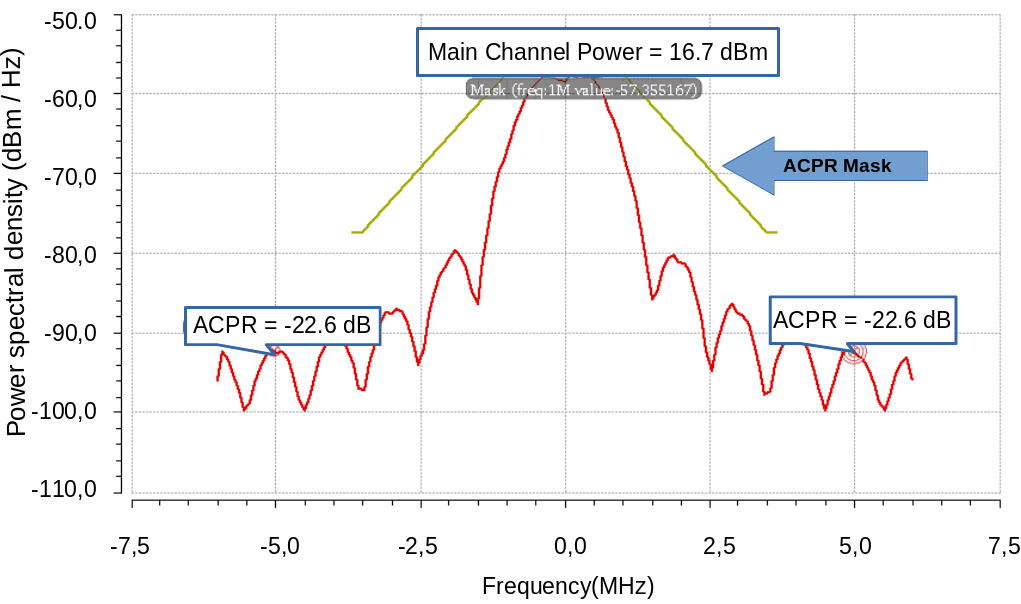
\includegraphics[width=7.4cm]{ex.png}
		 \caption{resposta ao degrau do motor em malha fechada com ganho unitário} \label{feedback1}
  		\end{center}
  	\end{figure}





	\begin{table*}
		\centering
		\caption{TABELA}
		\begin{tabular}[h]{r|cccc}
			\multicolumn{5}{c}{Leitura da balança (g)}\\
			\multicolumn{5}{c}{para cada largura da placa L}\\
			\hline
			I(A) & 100 milimetros & 50 milimetros & 25 milimetros & 12,5 milimetros\\
			     &   (g) &  (g) & (g) &  (g)\\
			\hline
			0,0 & 40,45 & 38,70 & 34,38 & 33,71 \\
			1,0 & 39,85 & 38,38 & 34,21 & 33,62\\
			2,0 & 39,53 & 37,90 & 33,97 & 33,45\\
			2,5 & 38,91 & 37,90 & 33,97 & 33,45\\
			3,0 & 38,60 & 37,77 & 33,87 & 33,41\\
			3,5 & 38,39 & 37,63 & 33,79 & 33,36\\
			4,0 & 38,00 & 37,48 & 33,71 & 33,32\\
			\hline
		\end{tabular}
	\end{table*}




	\lipsum[3]

	\section*{Conclusão}

	\lipsum[5-6]


	\bibliographystyle{IEEEtran}

	\bibliography{refes}

\end{document}